\documentclass[a4paper]{article}
\usepackage[utf8]{inputenc}
\usepackage[russian,english]{babel}
\usepackage[T2A]{fontenc}
\usepackage[left=10mm, top=20mm, right=18mm, bottom=15mm, footskip=10mm]{geometry}
\usepackage{indentfirst}
\usepackage{amsmath,amssymb}
\usepackage[italicdiff]{physics}
\usepackage{graphicx}
\usepackage{multirow}
\usepackage{svg}
\graphicspath{{images/}}
\DeclareGraphicsExtensions{.pdf,.png,.jpg}
\usepackage{wrapfig}
\usepackage{caption}
\captionsetup[figure]{name=Рисунок}
\captionsetup[table]{name=Таблица}
\title{\underline{Определение теплоемкости твердых тел}}
\author{Каспаров Николай, Б01-304}

\begin{document}

\maketitle
\begin{center}
\Large{\textbf{ }}
\end{center}

\subparagraph{Цель работы:}

\begin{enumerate}
    \item Прямое измерение кривых нагревания $T_{heat}(t)$
        и охлаждения $T_{cool}(t)$ пустого калориметра и системы 
        "калориметр + твердое тело";

    \item Определение коэффициента теплоотдачи стенок теплоотдачи стенок калориметра;

    \item Определение теплоемкости пустого калориметра и удельной теплоемкости твердого тела.

\end{enumerate}

\subparagraph{В работе используются:}

Калориметр, вольтметр, омметр, измеритель температуры - термопара,
источник питания, амперметр.

\section{Теоретическое введение}

В данной работе измерение теплоемкости происходит по стандартной схеме.
Исследуемое тело помезается в калориметр с нагревателем мощностью P.
Пусть за время $\Delta t$ к тело подвели $\Delta Q$ теплоты,
что привело к росту температуры на $\Delta T$,
тогда теплоемкость можно вычислить по данной формуле:

\begin{equation}
    C = \frac{\Delta Q}{\Delta T}
\end{equation}

Количество тепла, подведенная к системе не подчиняется формуле
$ \Delta Q \neq P \Delta t$, из-за тепловых потерь.
Верная формула выглядит так:

\begin{equation}
    C \Delta T = P \Delta t - \lambda \left( T - T_k \right) \Delta t
\label{eq:main}
\end{equation}

где $\lambda$ - коэффициент теплоотдачи стенок калориметра,
а $T_k$ - комнатная температура.

Из уравнения \eqref{eq:main} получим основные расчетные формулы работы.

\begin{equation}
    CdT = Pdt - \lambda \left[ T_{heat}(t) - T_k(t) \right]dt
\end{equation}
\begin{equation}
    CdT = - \lambda \left[ T_{cool}(t) - T_k(t) \right]dt
\end{equation}

\section{Методика эксперимента}

Температура измеряется термометром сопротивления.
Известно, что сопротивление проводника от времени изменяется по закону:

\begin{equation}
    R = R_{273} \left[ 1 + \alpha \left( T - 273 \right) \right],
\label{eq:R}
\end{equation}

где $R_{273}$ -- его сопротивление при $273\text{К}$,
а $\alpha$ -- температурный коэффициент сопротивления.

Выразим сопротивление $R_{273}$ через измеренное значение $R_k$.
Согласно \eqref{eq:R}, получаем:

\begin{equation}
    R_{273} = \frac{R_k}{1 + \alpha \left( T_k - 273 \right) }
\label{eq:R273}
\end{equation}

Подставляем \eqref{eq:R273} в \eqref{eq:R}, найдем:

\begin{equation}
    T(R_T) = 273 + \frac{R_T}{\alpha R_k}
            \left[1 + \alpha \left( T_k - 273 \right) \right] - \frac{1}{\alpha}
\end{equation}

Если считать, что $T_k = const$, то из (4) получим:

\begin{equation}
    \frac{CdT_{cool}}{- \lambda \left( T_{cool} - T_k \right) } = dt 
\end{equation}

После интегрирования получим зависимость:

\begin{equation}
    T_{cool}(t) = (T - T_k) e^{- \frac{\lambda }{C}t} + T_k
\label{eq:LC}
\end{equation}

Отсюда мы найдем $\lambda/C$.

Из уравнения (3) при $T_k = const$ получим:

\begin{equation}
    CdT_{heat} = Pdt - \lambda \left[ T_{heat} - T_k \right] dt
\end{equation}

После интегрирования получим зависимость:

\begin{equation}
    T_{heat}(t) = \frac{P}{\lambda} \left( 1 - e^{- \lambda t / C} \right) + T_k
\end{equation}

Отсюда найдем $\lambda$ и $C$.

\section{Построение графиков}

Для пустого калориметра получим:
\begin{equation*}
    \frac{\lambda_\text{к}}{C_\text{к}} = \left( 1.625 \pm 0.004 \right) 10^{-4} \text{с}^{-1}
\end{equation*}
\begin{equation*}
    \frac{P}{\lambda} = \left( 77.68 \pm 0.11 \right) \text{Дж}/\text{с}
\end{equation*}
\begin{equation*}
    C = (486 \pm 2) \text{Дж}/K
\end{equation*}

Для алюминия: 
\begin{equation*}
    \frac{\lambda_\text{а}}{C_\text{а}} = \left( 1.111 \pm 0.003 \right) 10^{-4} \text{с}^{-1}
\end{equation*}
\begin{equation*}
    \frac{P}{\lambda} = \left( 54.21 \pm 0.05 \right) \text{Дж}/\text{с}
\end{equation*}
\begin{equation*}
    C = (1019 \pm 3) \text{Дж}/K
\end{equation*}

Для титана:
\begin{equation*}
    \frac{\lambda_\text{т}}{C_\text{т}} = \left( 1.342 \pm 0.003 \right) 10^{-4} \text{с}^{-1}
\end{equation*}
\begin{equation*}
    \frac{P}{\lambda} = \left( 62.39 \pm 0.06 \right) \text{Дж}/\text{с}
\end{equation*}
\begin{equation*}
    C = (733 \pm 2) \text{Дж}/K
\end{equation*}

Соответствующие графики:
\begin{figure}[h!]
    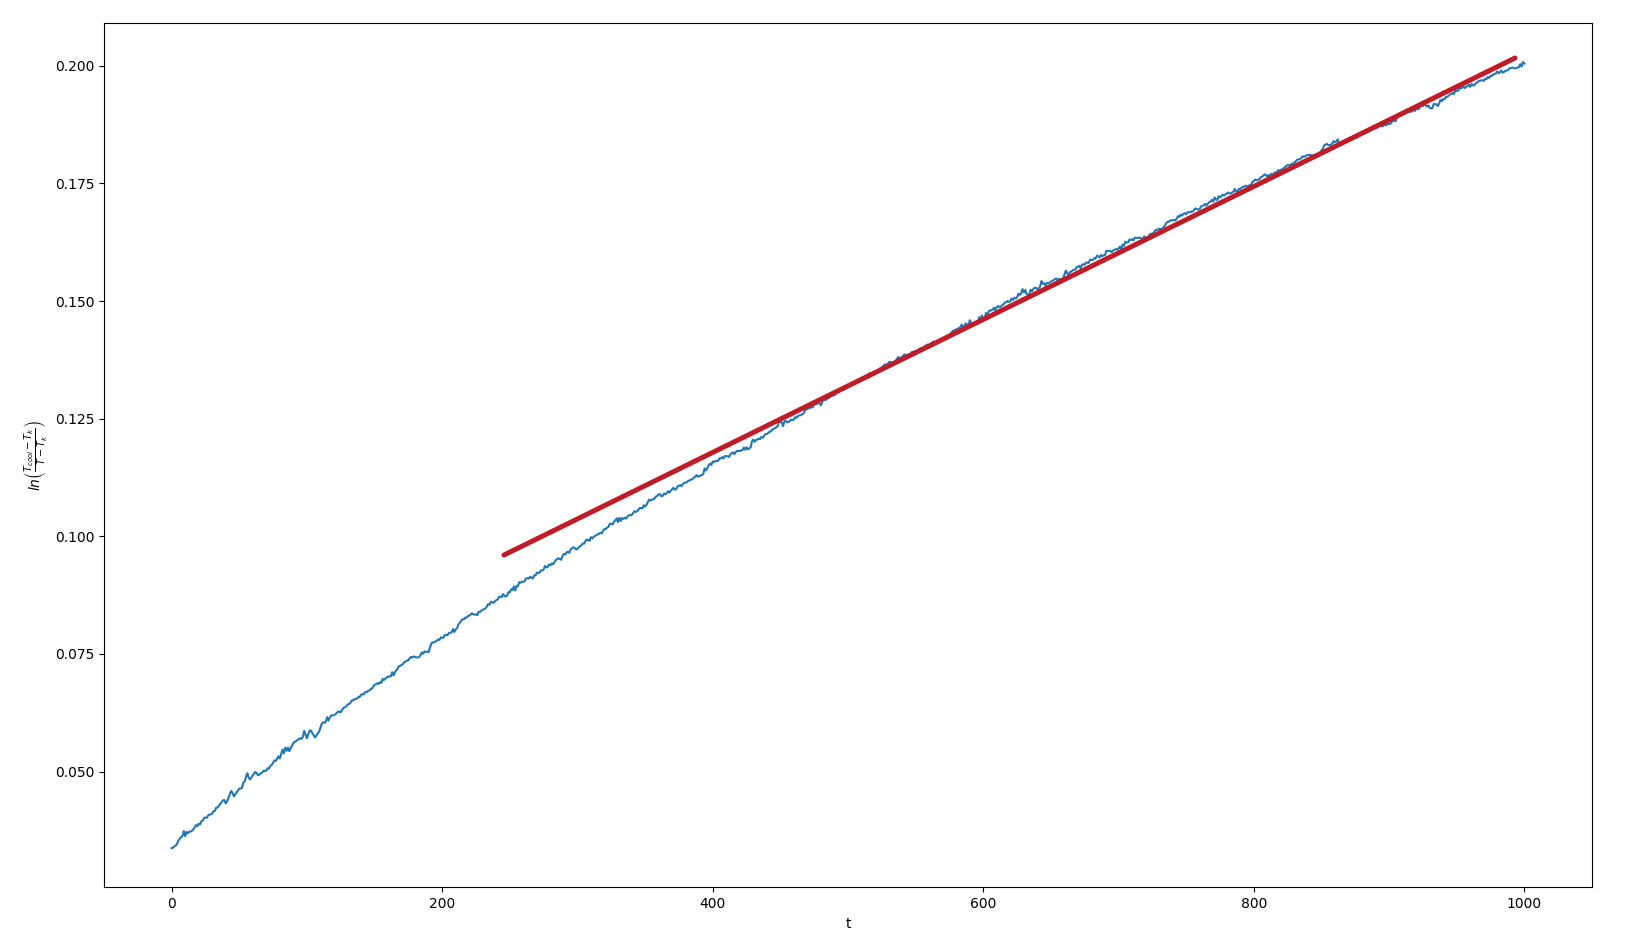
\includegraphics[scale=0.3]{empty.png}
    \caption{График остывания для пустого калориметра}
\end{figure}

\begin{figure}[h!]
    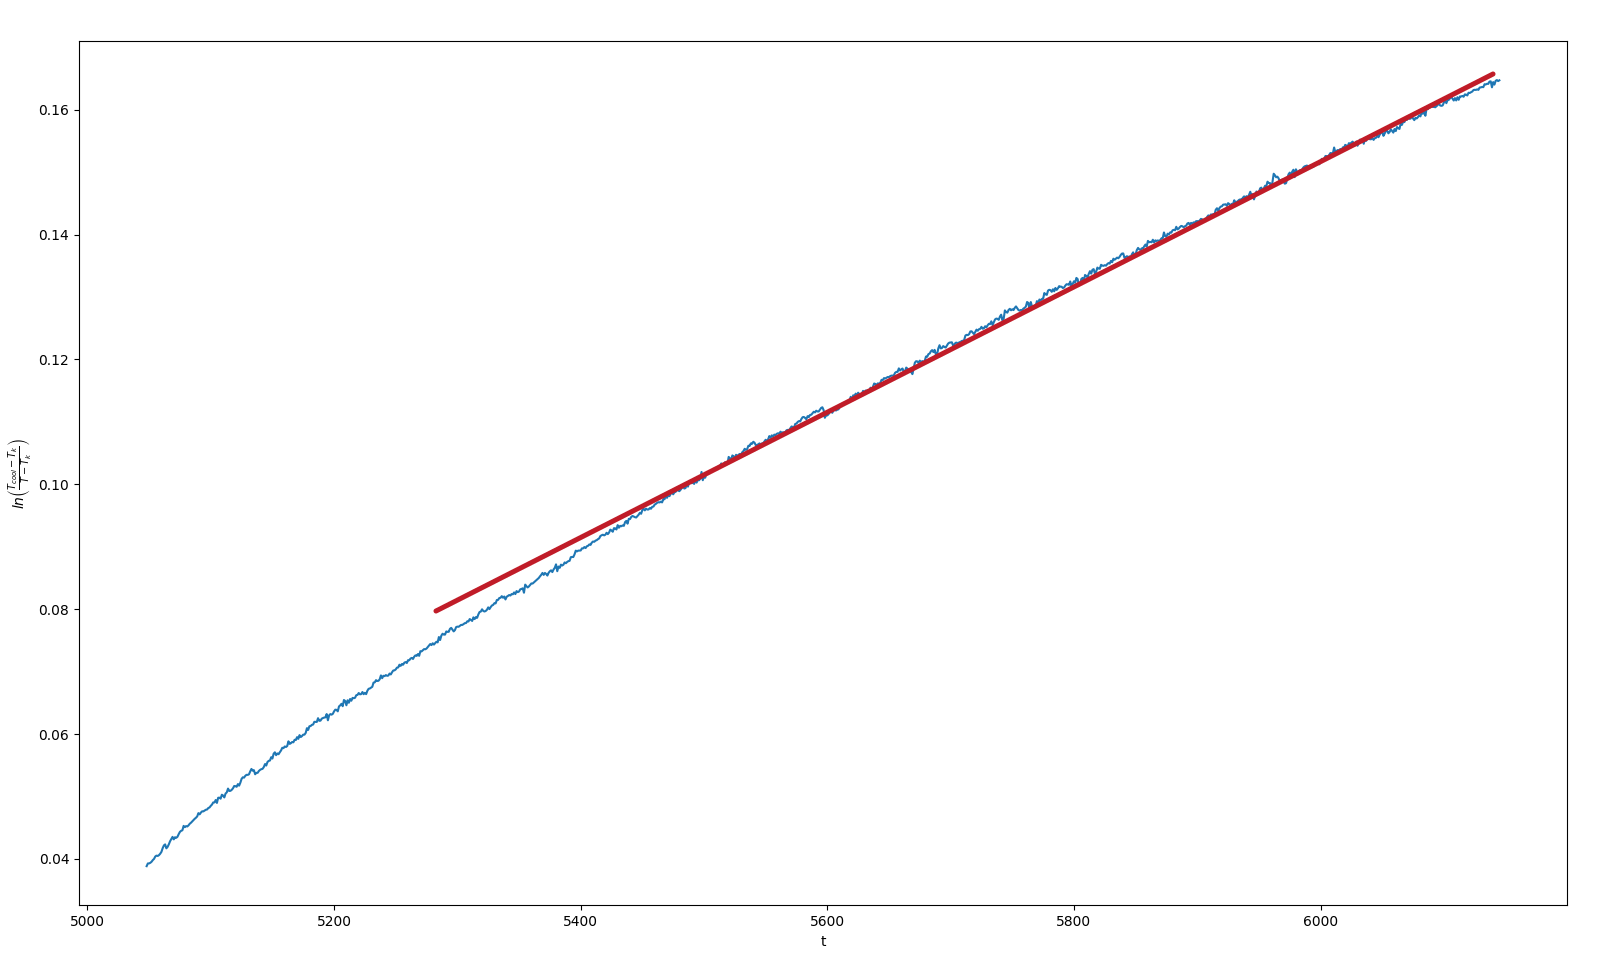
\includegraphics[scale=0.3]{alum.png}
    \caption{График остывания для алюминия}
\end{figure}

\begin{figure}[h!]
    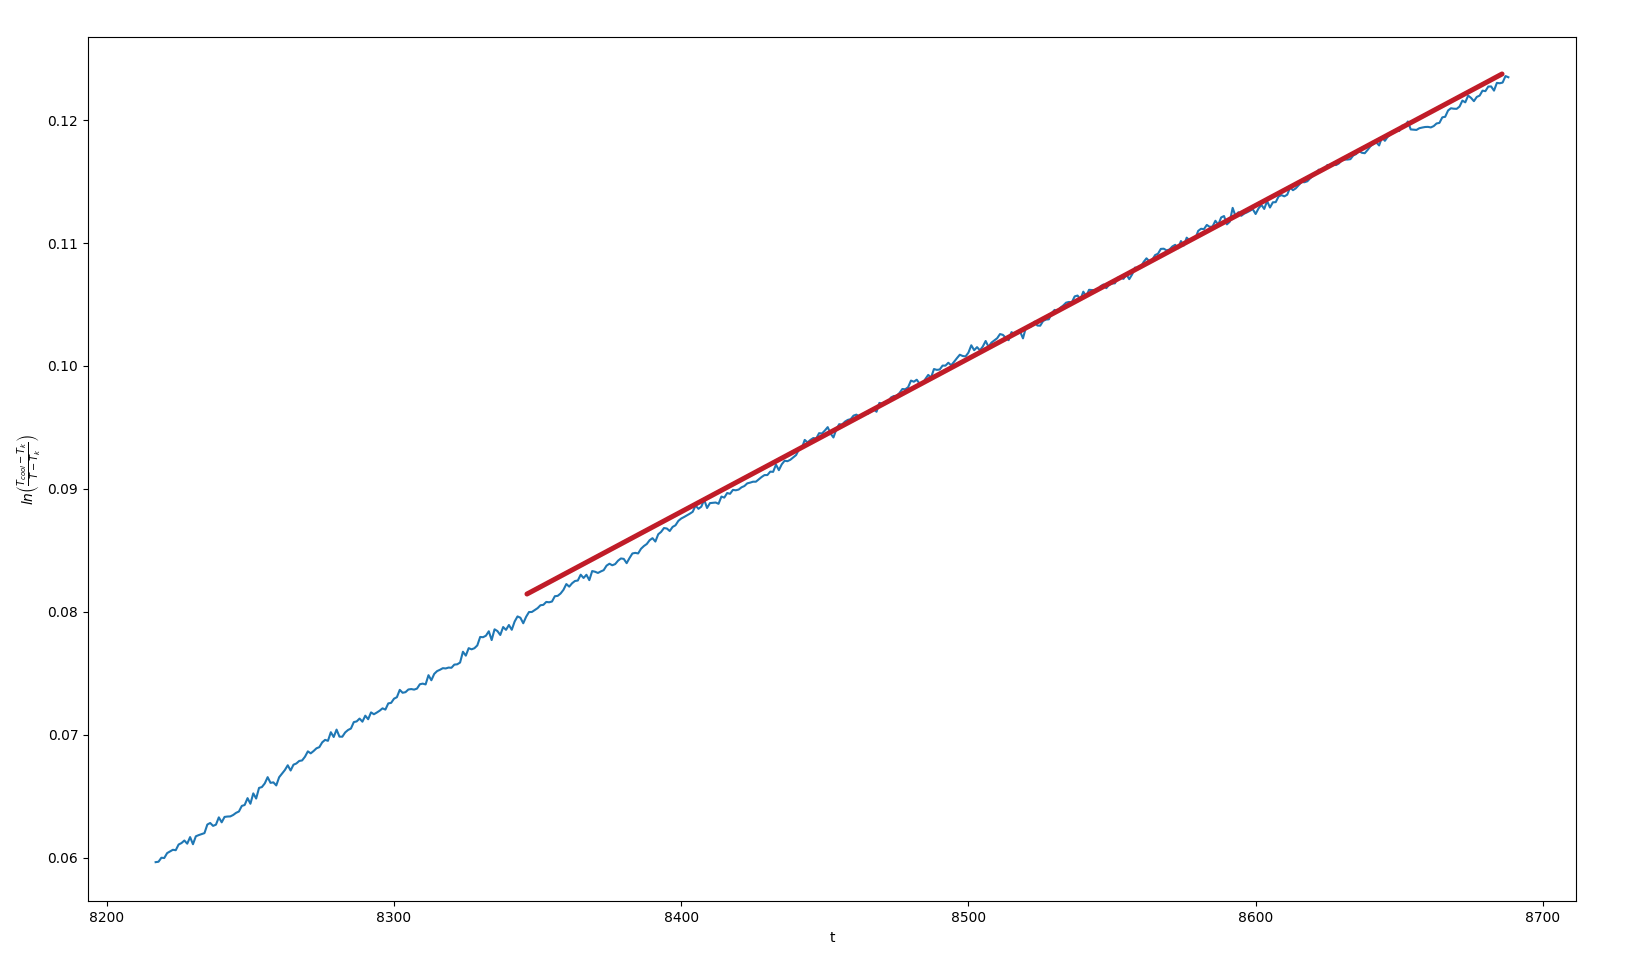
\includegraphics[scale=0.3]{tit.png}
    \caption{График остывания для титана}
\end{figure}

\begin{figure}[h!]
    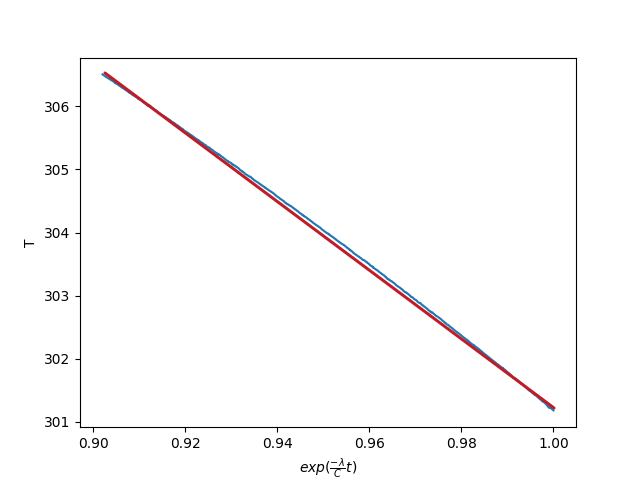
\includegraphics[scale=0.7]{lambda.png}
    \caption{График нагрева для алюминия}
\end{figure}

\begin{figure}[h!]
    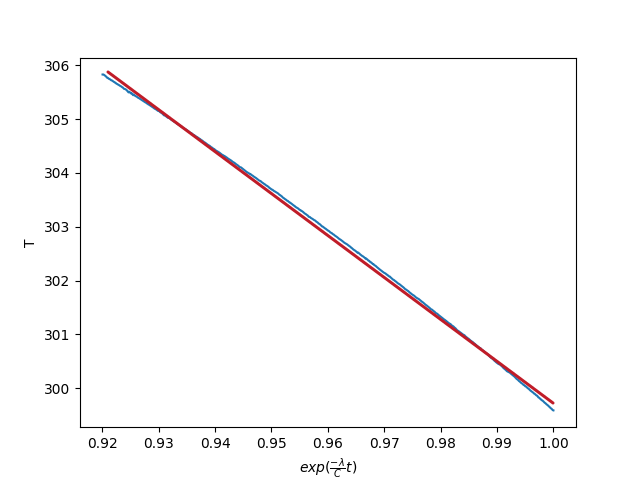
\includegraphics[scale=0.7]{pustoy.png}
    \caption{График нагрева для пустого калориметра}
\end{figure}

\begin{figure}[h!]
    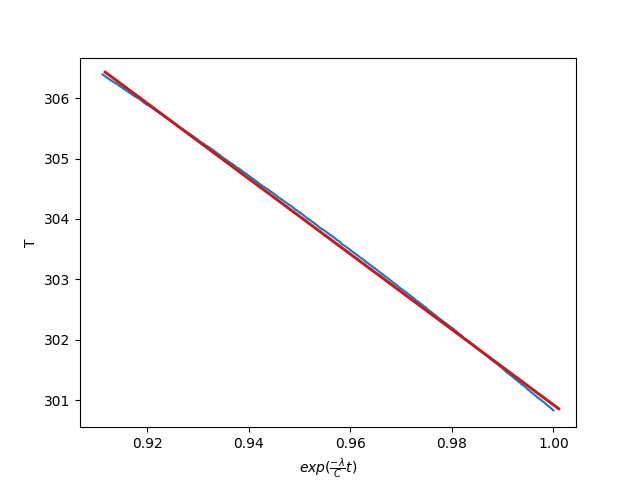
\includegraphics[scale=0.7]{titasd.png}
    \caption{График нагрева для титана}
\end{figure}

\clearpage

\section{Вывод}

Мы нашли отношения сопротивления проволоки от времени для процессов
нагревания и остужения пустого калориметра, титаного и алюминиего стержней.
Мы с довольно хорошей точностью смогли определить значения, которые не
совпали с табличными.

\begin{equation*}
    C_\text{а} = (533 \pm 5) \text{Дж}/K
\end{equation*}
\begin{equation*}
    C_\text{т} = (286 \pm 3) \text{Дж}/K
\end{equation*}

Точность эксперимента можно улучшить, улучшив стабильность комнатной температуры,
которую мы считали постоянной.

\end{document}
